% !TeX root = thesis.tex
\documentclass[
    11pt,
    a4paper,
    egregdoesnotlikesansseriftitles,
    toc=chapterentrywithdots,
    twoside,openright,
    titlepage,
    parskip=half,
    headings=normal,  % reduces heading size
    listof=totoc,
    bibliography=totoc,
    index=totoc,
    captions=tableheading,  % caption below table
    % chapterprefix,
    listof=flat,
    final
]{scrbook}

% details about your thesis
\newcommand{\titel}{Entwicklung eines Suchalgorithmusprototypen zur Bewertung von Suchergebnissen verschiedener Kategorien}
\newcommand{\artderarbeit}{Studienarbeit}  % {Bachelorarbeit,Masterarbeit}
\newcommand{\autor}{Marc Jonas Roser}
\newcommand{\studiengang}{Software Engineering}  % {Informatik,Wirtschaftsinformatik,Medieninformatik}
\newcommand{\matrikelnr}{364\,7316}
\newcommand{\erstgutachter}{Prof.\,Dr.~Hans-Georg Hopf}
\newcommand{\zweitgutachter}{}
\newcommand{\betreuer}{}
\newcommand{\unternehmen}{}
\newcommand{\logo}{figures/TH-Nuernberg-RGB.png}
\newcommand{\keywords}{}

% custom head and foot
\usepackage[automark]{scrlayer-scrpage}

\pagestyle{scrheadings}
\ihead{\headmark}
\chead{}
\ohead{\pagemark}
\renewcommand*\sectionmarkformat{
  \chapappifchapterprefix{\ }%
  \thechapter.\enskip
}

% Chapter and Section margins
% If needed adjust margins here to drastically increase pages ;)
\RedeclareSectionCommand[
  beforeskip=0\baselineskip,
  afterskip=.5\baselineskip]{chapter}
\RedeclareSectionCommand[
  tocindent=0pt,
  beforeskip=0.5\baselineskip,
  afterskip=.1\baselineskip]{section}
\RedeclareSectionCommand[
  tocindent=10pt,
  beforeskip=-.25\baselineskip,
  afterskip=0.1\baselineskip]{subsection}

\usepackage{scrhack}

% other packages
\usepackage[utf8]{inputenc}
\usepackage[T1]{fontenc}
\usepackage{lmodern,relsize,textcomp,csquotes}
\usepackage{amsfonts}
\usepackage[ngerman,english]{babel}  % flip for German thesis
\usepackage{caption}
\usepackage{subcaption}
\DeclareCaptionFormat{custom}
{%
    \textbf{#1#2}\textit{\small #3}
}
\captionsetup{format=custom}
\usepackage{graphicx}
\usepackage{wrapfig}
\usepackage{setspace,geometry,xcolor}
\usepackage{makeidx}
\usepackage{url}
\usepackage[toc]{glossaries}
\usepackage{pdfpages}

% table setup
\usepackage{longtable}
\usepackage{array}
\usepackage{ragged2e}
\usepackage{lscape}

% pdf hyperref
\usepackage[
    bookmarks=true,
    bookmarksopen=true,
    bookmarksnumbered=true,
    bookmarksopenlevel=1,
    pdftitle={\titel},
    pdfauthor={\autor},
    pdfcreator={\autor},
    pdfsubject={\titel},
    pdfkeywords={\keywords},
    pdfpagelabels=true,
    colorlinks=true,
    linkcolor=black,
    urlcolor=magenta,
    anchorcolor=black,
    citecolor=cyan,
    filecolor=magenta,
    menucolor=red,
    plainpages=false,
    hypertexnames=true,
    linktocpage=true,
    linktoc=all,
    % hidelinks Uncomment in Production build
]{hyperref}

% page setup
% \setlength{\topskip}{\ht\strutbox}
\geometry{paper=a4paper,left=2.5cm,top=3.0cm,bindingoffset=.8cm}
\onehalfspacing
\frenchspacing
\clubpenalty = 10000
\widowpenalty = 10000
\displaywidowpenalty = 10000

% Uncomment to enable better printing support
% \clearpage
% Comment to enable better printing support
\let\cleardoublepage=\clearpage

% load glossary entries
\makenoidxglossaries
\loadglsentries{glossary}

% Remove hbox errors
\hfuzz=7.5pt

\begin{document}

\setcounter{secnumdepth}{3}  % numerate subsections
\setcounter{tocdepth}{2}  % ...but don't include them in toc

\frontmatter
\pagenumbering{Roman}
\thispagestyle{empty}
\pdfbookmark[1]{Cover}{cov}
\begin{titlepage}

\begin{center}

\includegraphics[width=\linewidth]{figures/TH-Nuernberg-RGB.png}\\[1cm]
\LARGE{Fakultät Elektrotechnik Feinwerktechnik Informationstechnik}\\[2cm]

\huge
\textbf{\titel}\\[1cm]
%
\Large
\artderarbeit~im Studiengang \studiengang\\[1cm]
%
\large
vorgelegt von

\Large
\autor\\[0.5cm]
\small
Matrikelnummer \matrikelnr\\[2cm]

\vspace*{\fill}

\large
\begin{tabular}{p{3cm}p{8cm}}\\
Erstgutachter:  & \quad \erstgutachter\\[1.2ex]
Zweitgutachter: & \quad \zweitgutachter\\[1.2ex]
%discomment "Betreuer" and "Unternehmen" for a thesis in a company
%Betreuer: & \quad \betreuer\\
%Unternehmen: & \quad \unternehmen
\end{tabular}
\end{center}

\begin{center}
\copyright\,\the\year
\end{center}

\vspace{-0.5cm}
\singlespacing
\small
\noindent Dieses Werk einschließlich seiner Teile ist \textbf{urheberrechtlich geschützt}.
Jede Verwertung außerhalb der engen Grenzen des Urheberrechtgesetzes ist ohne Zustimmung des Autors unzulässig und strafbar.
Das gilt insbesondere für Vervielfältigungen, Übersetzungen, Mikroverfilmungen sowie die Einspeicherung und Verarbeitung in elektronischen Systemen.

\end{titlepage}

\thispagestyle{empty}
\section*{Kurzdarstellung}
\label{sec:kurzdarstellung}
Das Ziel der vorliegenden Studienarbeit ist es, eine bestehende Datenbank mit multimedialen Inhalten möglichst effizient nach unterschiedlichen Kriterien zu durchsuchen.
Suchergebnisse sollen nach bestimmten Kriterien gewichtet, gefiltert und sortiert werden. Vorschläge für eine weiterführende Navigation auf der Suchergebnisseite sollen angeboten werden, Suchergebnisse sollen dazu nach Kontext und Wahrscheinlichkeiten gewichtet angezeigt werden.
Das theoretische Fundament dieser Arbeit stellt die wissenschaftliche Betrachtung der Methoden zur Bewertung der Relevanz von Suchergebnissen dar. Die Arbeit untersucht die Möglichkeit, einen Suchbegriff so zu analysieren, dass ein Nutzer die bestmögliche Ergebnisliste bzw. zielgerichtete weiterführende Navigationsmöglichkeiten erhält.
Die bestehende Anwendung "\gls{crossload}" wird vorgestellt, um dem Leser einen Kontext zu bieten, in der sich die Entwicklung bewegt.

\section*{Abstract}
\label{sec:abstract}
The goal of this student research project is to search an existing database with multimedia content as efficiently as possible according to various criteria.
Search results are to be weighted, filtered, and sorted according to certain criteria. Suggestions for further navigation on the search results page are to be offered, and search results are to be displayed weighted according to context and probabilities.
The theoretical foundation of this work is the scientific consideration of methods for evaluating the relevance of search results. The work examines the possibility of analyzing a search term in such a way that a user receives the best possible list of results or targeted further navigation options.
The existing application "Crossload" is presented to provide the reader with a context in which the development takes place.

\clearpage
\section*{Eidesstattliche Erklärung}
\label{sec:explanation}
Hiermit versichere ich, Marc Jonas Roser, ehrenwörtlich, dass ich die vorliegende Studienarbeit mit dem Titel: „Entwicklung eines Prototypen eines Suchalgorithmus zur Bewertung von Suchergebnissen verschiedener Kategorien“ selbstständig und ohne fremde Hilfe verfasst und keine anderen als die angegebenen Hilfsmittel benutzt habe. Die Stellen der Arbeit, die dem Wortlaut oder dem Sinn nach anderen Werken entnommen wurden, sind in jedem Fall unter Angabe der Quelle kenntlich gemacht. Die Arbeit ist noch nicht veröffentlicht oder in anderer Form als Prüfungsleistung vorgelegt worden.
Ich versichere zudem, dass die eingereichte elektronische Fassung mit der gedruckten Fassung übereinstimmt.

Nürnberg, 25.09.2022

Marc Jonas Roser

\tableofcontents
\printnoidxglossaries

\mainmatter
\chapter{Einleitung}\label{ch:intro}

\section{Relevanz des Themas}
Suchalgorithmen und relevante Suchergebnisse sind derzeit so relevant wie noch nie.
Dabei wollen die Benutzer einer Suchmaschine in Sekundenbruchteilen Ergebnisse, die am besten zu ihrem Suchbegriff passen, ohne sich dabei viel Gedanken über die Formulierung eines solchen Begriffes zu machen.
Ein Beispiel für einen solchen Algorithmus ist Google, welches seit den frühen 2000ern einen kometenhaften Aufstieg in der Welt der Suchmaschinen hinter sich hat, was anhand der erreichten Werbeeinnahmen sichtbar wird.\footnote{Siehe \ref{fig:werbeumsatz}}
Google ist im Vergleich zu anderen Suchmaschinen so stark verbreitet\footnote{Siehe \ref{fig:marketshare}}, dass mittlerweile sogar der Duden das Verb „googeln“ als eigenen Begriff für die Recherche im Internet führt.\footnote{Vgl. Duden \cite{duden2022}}
Dabei stellt sich für die Entwicklung eigener Produkte die Frage, wie aus einem Suchbegriff, der meist nur aus wenigen Wörtern bis zu einem ganzen Satz besteht, relevante Suchergebnisse gefunden werden können. Dies würde zur Akzeptanz der Nutzer im Hinblick auf die entwickelte Funktionalität führen, da gewünschte Ergebnisse schneller und ohne großen Aufwand gefunden werden können.

\section{Ausgangssituation}
Derzeit besteht bei \gls{crossload}\footnote{Siehe Crossload.org \cite{pfleiderer2022}}, einer Plattform zum Durchsuchen und Anhören einer umfassenden Predigt Datenbank, eine Datenbank mit einer Such \gls{api} auf Basis von Spring Boot und \gls{solr}. Diese teilt auf der Suchergebnisseite die Ergebnisse nach Kategorien auf und somit können nur schwer übergreifende Suchanfragen getätigt werden. Zwar werden alle Treffer auf der gleichen Seite angezeigt, doch durch die Aufteilung nach Kategorien werden Ergebnisse gewisser Kategorien über anderen gezeigt, auch wenn niedrig positionierte Kategorien relevantere Ergebnisse enthalten.

\section{Zielsetzung}
Das Ziel der vorliegenden Studienarbeit ist es durch eine theoretische Betrachtung der Bewertung der Relevanz von Suchergebnissen und der anschließenden Entwicklung eines Prototyps, ein bestehendes Produkt zu erweitern. Diese Erweiterung umfasst, die nach Kontext und Wahrscheinlichkeiten gewichtete und gefilterte Suche über eine Datenbank mit Datentypen verschiedener Kategorien bei der zusätzlich Vorschläge zur weiteren Navigation auf der Suchergebnisseite gegeben werden sollen.

\chapter{Grundlagen}
\label{ch:grundlagen}

\section{Relevanz}

Relevanz ist allgemein beschrieben eine Beziehung zwischen einem Individuum, dem zeitlichen Rahmen, in welchem dieses eine Information benötigt und einer beliebigen Information.\footnote{vgl. Bookstein S. 1 \cite{bookstein2007}}
Das bedeutet, dass Relevanz von Person zu Person unterschiedlich ist, da zum einen diverse Informationen nur zu einer bestimmten Zeit notwendig bzw. wichtig sind und der Kontext der benötigten Information sich ständig ändert.

% Relevant Search ab Seite 6 (PFD: 31)
% TODO: Absätze über Information Retrieval by Christopher D. Manning Was ist Informationsgewinnung, Was hat Relevanzz damit zu tun

\section{Relevanz von Suchergebnissen und Methoden zur Bewertung}

Eine \gls{searchEngine} gibt nach Anfrage Websiten sortiert nach der Relevanz der Ergebnisse abhängig zum gegebenen Suchbegriff des Nutzers.
Die Schwierigkeit dabei, ist die Bestimmung der Relevanz für eine beliebige Website.
Moderne Suchmaschinen nutzen dutzende oder gar hunderte verschiedener Methoden um Features um die Relevanz der verfügbaren Suchergebnisse zu bewerten.
Die spezifischen Funktionen und Methoden werden von den Unternehmen geheim gehalten, um einen Missbrauch ihrer \gls{searchEngine} zu verhindern.
Dennoch sind die am häufigsten genutzten Merkmale bekannt und in einigen wissenschaftlichen Arbeiten untersucht worden.\footnote{vgl. Zaragoza, Najork, S. 1 \cite{zaragoza2018}}

Zur Einfachheit wird von der Webapplikation \gls{crossload} abstrahiert und stattdessen Beispiele aus der Internetsuche verwendet, welche zum Beispiel mit Google, Bing, Ecosia oder anderen \gls{searchEngine}n üblich ist.

\subsection{Textuelle Relevanz}
Das einfachste Merkmal für die Bewertung der Relevanz ist den kompletten Inhalt nach der textuellen Relevanz zu bewerten.
Da natürliche Sprache, die meist für Suchergebnisse genutzt wird, generell ungenau ist, wird mit sogenannten "Matching Functions" versucht auch ungefähre Übereinstimmungen in einem Fliesstext zu finden.
Einige der verwendeten Funktionen um die textuelle Relevanz zu bewerten sind dabei\footnote{vgl. Zaragoza, Najork, S. 1 \cite{zaragoza2018}}

\begin{itemize}
  \item Die Anzahl der Treffer für den Suchterm oder Abwandlungen
  \item Position des Suchterms (früheres Vorkommen)
  \item Seiten Struktur (für Websiten: Ist der Term eine Überschrift o.ä.)
  \item Grafisches Layout (für Websiten: Ist der Term z.B. farblich markiert)
\end{itemize}
\subsection{Relevanz durch Attribute}

\subsection{Hyperlink Relevanz}

\subsection{Relevanz durch Nutzerverhalten}

\subsection{Performance}

\subsection{Personalisierung}

\subsection{Kombination}

\chapter{Anforderungen und Problemanalyse}
\label{ch:anforderungen}

Im folgenden Kapitel sollen alle wesentlichen Funktionen des geplanten Prototyps dargestellt werden.
Da es sich um ein kleines Projekt mit einem abgestecktem Rahmen handelt und es kein Team gibt, welches die Entwicklung durchführt, wird das Wasserfallmodell für diese Entwicklung verwendet.\footnote{Vgl. \ref{sec:methods}}


\section{Vorgehensweise}
\label{ref:requirementMethods}
Zur Erfassung der Anforderungen bzw. Requirements Engineering werden User Stories benutzt. Diese sind bekannt aus agilen Softwareentwicklungsmodellen, wie z. B. Scrum, entstanden aber durch praktische Erfahrungen in der Softwareentwicklung.
Konzeptioniert wurden sie von Dr. Ivar Jacobsen\footnote{Vgl. Jacobson, Spence, Kerr 2016 \cite{jacobson2016}} und Ron Jeffries\footnote{Vgl. Ron Jeffries \cite{jeffries2022}}.
Mithilfe einfacher Sprache wird aus der Sicht des Stakeholders das Ziel einer Story in einem kurzen Satz zusammengefasst.
Anschließend wird dieses Ziel begründet, um die Wichtigkeit und Existenzberechtigung der Story zu begründen.
User Stories sind dabei auch Anforderungen nach dem SMART Prinzip\footnote{Vgl. Witte 2019a, S. 67 \cite{witte2016}}, da diese nur einen sehr kleinen abgesteckten Teilbereich einer Funktionalität enthalten.
Dadurch sind sie einfacher schätzbar, umsetzbar und testbar. Anhand der ermittelten User Stories werden nach der Entwicklung Akzeptanztests durchgeführt, um den Erfolg des Endproduktes objektiv zu bewerten.

\section{User Stories}
\label{sec:userStories}
Die Anforderungen umfassen alle Aktionen, welche der Nutzer in der Anwendung durchführen will.
Ziel aller Anforderungen ist die übergreifende Suche über mehrere Kategorien effizient anhand mehrerer Kriterien zu durchsuchen und zu bewerten.
Anhand dieses Ziels werden User Stories entwickelt, in denen ein Nutzer und andere Personen ihre Anforderungen an das zu entwickelnde Produkt stellen.

Nichtfunktionale Anforderungen werden bei dieser Anforderungserhebung nicht beachtet, da es sich hierbei um die Erweiterung einer bestehenden \gls{api} handelt und Aspekte wie Benutzerfreundlichkeit und User Experience hierbei wenig relevant sind, bzw. das Entwicklungsumfeld durch die bereits bestehende Anwendung vorgegeben ist.
Die Priorität der einzelnen User Stories ergibt sich aus der unten gegebenen Reihenfolge.

\pagebreak
Ich, als Benutzer, will …
\begin{itemize}
  \item[…] für ein gegebenes Suchkriterium relevante Suchergebnisse über mehrere Kategorien hinweg erhalten, damit mit einer einzelnen Suche nur eine geringe Teilmenge der Datenbank angezeigt wird.
  \item[…] die erhaltenen Suchbegriffe nach Kontext und Wahrscheinlichkeit gewichtet erhalten, damit diese im späteren Verlauf sortiert werden können. Der Kontext ergibt sich aus möglichen Schlagworten, die im Suchbegriff verwendet worden, womit z. B. eine Kategorie, ein Attribut eines Ergebnisses oder höher gewertet wird. Beispiele wären:
    \begin{itemize}
      \item[…] der Titel eines Buches wird „relativ“ genau als Suchbegriff eingegeben, folglich wird dieses Buch stärker gewichtet.
      \item[…] der Suchbegriff enthält den Term „Video“, folglich werden alle Videos priorisiert.
    \end{itemize}
  \item[…] die erhaltenen Suchbegriffe anhand des errechneten Gewichts absteigend sortiert zurückgegeben bekommen, damit das relevanteste Suchergebnis auf der Suchergebnisseite ganz oben steht.
  \item[…] ein mit hoher Wahrscheinlichkeit gesuchtes Suchergebnis als Vorschlag angezeigt bekommen, damit auf der Suchergebnisseite eine schnelle Navigation zu diesem Ergebnis möglich ist.
    Dabei soll ein Inhalt nur vorgeschlagen werden, wenn dessen Relevanz um einiges höher ist, als das der anderen gefundenen Ergebnisse.
    Dies verhindert, dass von ähnlich relevanten Suchergebnissen eines ohne Berechtigung hervorgehoben wird, auch wenn es das Relevanteste in dieser Liste ist.
\end{itemize}

\chapter{Konzeption}
\label{ch:conception}


\section{Analyse der Arbeitspakete}
\section{Konzeption}

\chapter{Entwicklung des Prototyps}
\label{ch:development}

Die Umsetzung des Prototyps erfolgt in mehreren Schritten. Zu Beginn wird wie in \ref{sub:unifiedList} beschrieben, die Liste aller Ergebnisse zusammengeführt und absteigend nach der Relevanz sortiert. Anschließend wird der Schlagwortabgleich (\ref{sub:keyword}) implementiert, indem konfigurierbar die Liste der möglichen Synonyme mit dem Suchterm abgeglichen wird und die Ergebnisse geboostet werden, wenn der Suchterm ein Synonym enthält. Zuletzt werden die resultierenden Inhalte nach einem möglichen Vorschlag wie in \ref{sub:suggestion} beschrieben dem Ergebnis hinzugefügt.

\section{Zusammengeführte Liste}
\label{sec:devUnifiedList}

% TODO: Crossload Frontend Suchseite nicht in Kategorien, sondern Komplett.
% TODO: Änderungen zusammenfassen https://gitlab.crossload.org/crossload/frontend/frontend/-/tree/studienarbeit


\section{Schlagwortabgleich}
\label{sec:devKeywords}

% TODO Create configurable JSON mit ausgearbeiteten Schlagwörtern
% TODO For each configuration: Search for Keywords in Search Term
% TODO If found, boost Contents with Category


\section{Vorschläge für weitere Navigation}
\label{sec:devSuggestions}

% TODO Adjust Schema, -> add suggestion object
% TODO Create Function to determine suggestion
% TODO Add Suggestion to result

\chapter{Auswertung}
\label{ch:evaluation}
Ziel des Prototyps war es, für die Website Crossload relevantere Inhalte in der Suche herauszufiltern und anzuzeigen.
Im Verlaufe dieses Kapitels werden die konzeptionierten und entwickelten Ergebnisse anhand dieses Ziels genauer untersucht.

Anhand des Prototyps und den erhobenen funktionalen Anforderungen kann einfach festgestellt werden, inwiefern diese Funktionalitäten für den Nutzer möglich sind.
Für den Abgleich dieser Funktionalitäten wird für jede Anforderung ein kurzer Titel gegeben, der Status, ob diese erfüllt wurde oder nicht, sowie falls eine Begründung oder Zwischenstand der Bearbeitung.

\begin{longtable}{p{0.25\textwidth}|c|p{0.5\textwidth}}
  \label{tab:requirements}\\
  \textbf{Anforderung} & \textbf{Status} & \textbf{Begründung} \\
  \hline
  \hline
  Gemischte Suchergebnisse über alle Kategorien & Erledigt & Suchergebnisse werden zusammengeführt auf der Suchergebnisseite angezeigt. \\
  \hline

  Relevanz für ähnliche Schlagwörter & Gegeben & Ähnliche Suchtitel werden bereits durch *-Zeichen in der gegebenen Suche gefunden (Vgl. \ref{code:SOLRSuggestionQuery}). \\
  \hline

  Relevanz anhand von Kategorien & Erledigt & Für eingegebene Kategorien werden ähnliche Inhalte um ein vielfaches geboostet. \\
  \hline

  Nach Relevanz absteigende Sortierung & Gegeben & Sortierung und Richtung bereits auf Suchergebnisseite gegeben \\
  \hline

  Vorschläge & Erledigt & Der relevanteste Vorschlag wird von der Suche herausgefiltert und falls gefunden, auf der Suchergebnisseite angezeigt. \\
  \caption{Anforderungsanalyse}
\end{longtable}

Der endgültige Stand aller funktionalen Anforderung kann in folgenden Kennzahlen zusammengefasst werden:
\begin{itemize}
  \item 3 von 5 Anforderungen wurden erfüllt.
  \item 2 von 5 Anforderungen waren bereits gegeben und wurden nicht verändert.
\end{itemize}

\chapter{Diskussion der Ergebnisse}
\label{ch:discussion}

\section{Abgleich der Ergebnisse mit den gestellten Anforderungen}
\section{Identifizierte Probleme}
\section{Bewertung}

\chapter{Ausblick}
\label{ch:summary}


\backmatter
\pagenumbering{Roman}
% \renewcommand{\thechapter}{\Alph{chapter}}
% \renewcommand{\thesection}{\Roman{section}}
% \renewcommand{\thesubsection}{\Roman{section}}
\appendix

\pagenumbering{Alph}
\renewcommand{\thechapter}{\Alph{chapter}}
\renewcommand{\thesection}{\Roman{section}}
\renewcommand{\thesubsection}{\Roman{section}}

\chapter{Anhang}
\label{appendix:annex}

\section{Bilder}
\begin{wrapfigure}{l}{\textwidth}
  \begin{centering}
    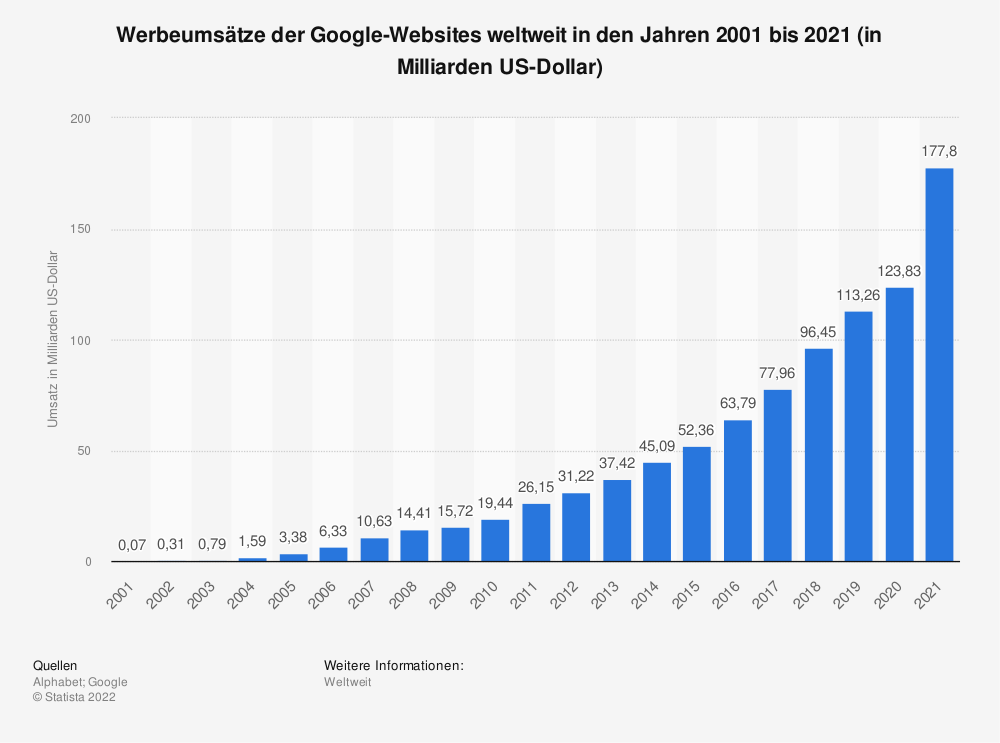
\includegraphics[width=.8\textwidth]{figures/appendix/werbeumsatz.png}
    \caption{Werbeumsätze Google Websites \cite{alphabet2022}}
    \label{fig:werbeumsatz}
  \end{centering}
\end{wrapfigure}

\begin{wrapfigure}{r}{\textwidth}
  \begin{centering}
    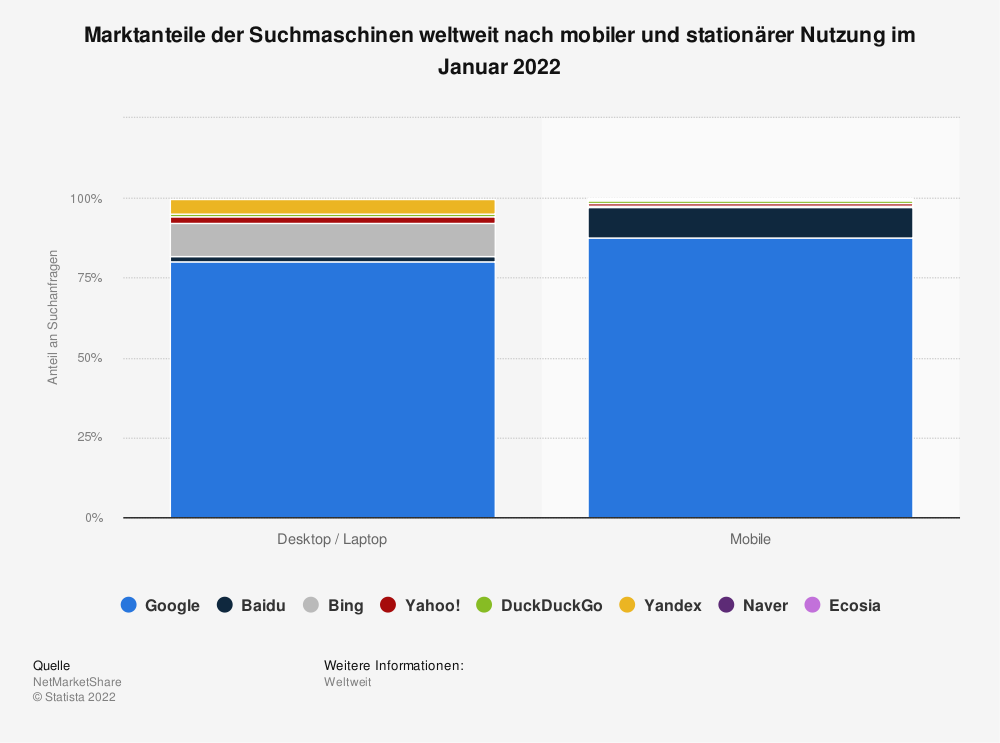
\includegraphics[width=.8\textwidth]{figures/appendix/marketshare.png}
    \caption{Marktanteil Google \cite{netmarketshare2022}}
    \label{fig:marketshare}
  \end{centering}
\end{wrapfigure}

\begin{wrapfigure}{r}{\textwidth}
  \begin{centering}
    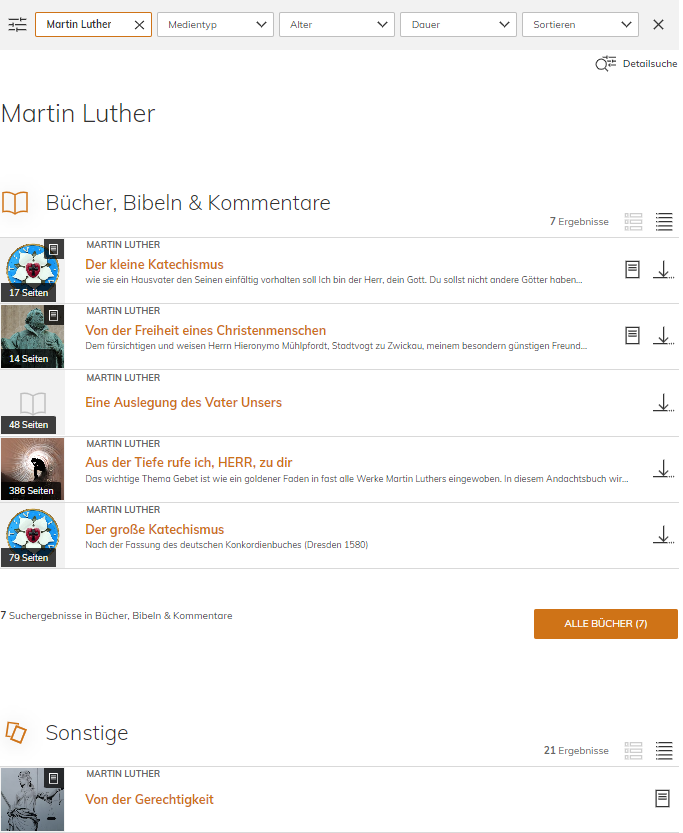
\includegraphics[width=.8\textwidth]{figures/appendix/crossloadSuche.png}
    \caption{Crossload \cite{pfleiderer2022}}
    \label{fig:crossloadSuche}
  \end{centering}
\end{wrapfigure}


% 2 Images on one page
% \begin{figure}
%   \includegraphics[width=\textwidth]{figures/appendix/IMAGE.png}
%   \caption{\label{fig:IMAGE} TITLE \cite{CITATION}}
%   \includegraphics[width=\textwidth]{figures/appendix/IMAGE.png}
%   \caption{\label{fig:IMAGE} TITLE \cite{CITATION}}
% \end{figure}

% 1 Images per page
% \begin{figure}
%   \includegraphics[width=\textwidth]{figures/appendix/IMAGE.png}
%   \caption{\label{fig:IMAGE} TITLE \cite{CITATION}}
% \begin{figure}
% \end{figure}
%   \includegraphics[width=\textwidth]{figures/appendix/IMAGE.png}
%   \caption{\label{fig:IMAGE} TITLE \cite{CITATION}}
% \end{figure}

\listoffigures
\listoftables
\bibliographystyle{ieeetr}
\bibliography{refs}

\end{document}
